\documentclass[10pt]{article}
\usepackage[utf8]{inputenc}
\usepackage{url}
\usepackage{hyperref}
\usepackage{amsmath}
\usepackage{amssymb}
\usepackage{graphicx}
\usepackage{multicol}
\usepackage{enumitem}
\usepackage[font=small]{caption}

\addtolength{\textfloatsep}{-5mm}
\setlength\columnsep{20pt}
\usepackage[a4paper,left=1.50cm, right=1.50cm, top=1.50cm, bottom=1.50cm]{geometry}

\author{}

\title{Semester Project Report}

\begin{document}
\begin{center}
    {\Large \textbf{The Movie Database \\ Or: How I Learnt to Visualize Data}}\\
    \vspace{1em}
    {\large Nabin Kumar Sahoo}\\
    \vspace{1em}
    \textit{Chennai Mathematical Institute}
\end{center}
\begin{center}
    \rule{165mm}{0.2mm}
\end{center}

\begin{abstract}
This is the final report of the semester project of the Visualisation course taken during August-November, 2022 at Chennai Mathematical Institute. 

The purpose of the project is to study and analyse 
the quantitative aspects of movies, like average rating, budget, runtime, among other variables.
We also aim to study relations among different genres.

The visualisation is done in \texttt{R} using the \texttt{ggplot2} package. 
\end{abstract}

\begin{center}
    \rule{165mm}{0.2mm}
\end{center}

\begin{multicols}{2}

\section{Introduction}

Cinema is, and has been since early 20th century, one of the most prevelant forms of art. 
The visual basis of the medium gives it a universal power of communication, 
and its reach is easily extended (by breaking language barriers) through the use of subtitles or dubbing.

Being a huge -- pardon my presumption -- movie afficionado, I can say that movies have been an essential part of my life.

\subsection{Project Description}
Through this project I will explore the quantitative aspects of movies -- 
average rating (out of 10), budget, vote counts, runtime -- 
and the relationships among them.
Specifically, I will study the following relations:  
\begin{itemize}
    \item \emph{Avg. rating vs Budget}, 
    \item \emph{Avg. rating vs Genre}, 
    \item \emph{Avg. rating vs Runtime}, and
    \item \emph{Budget vs Genre}.
\end{itemize}

I will also explore the relationship among different genres. 
Often, as is understandable, a particular movie doesn't have only one genre attributed to it, instead there are usually two or three (or even more) genres. 
For example, \emph{Quantum of Solace (2003)} has four genres, namely \emph{Adventure}, \emph{Action}, \emph{Thriller}, and \emph{Crime}.
So, I will look at what (co-)genres are most common with what genres. 



\section{Dataset}

The dataset used is the \textbf{TMDb (The Movie Database) 5000}\footnote{\url{https://www.kaggle.com/datasets/tmdb/tmdb-movie-metadata}} dataset, generated from TMDb API.
It has data on more than 4800 movies.

There are two csv files, \texttt{tmdb\_5000\_credits.csv} and \texttt{tmdb\_5000\_movies.csv}. 
For now, we will solely work with the latter.

\subsection{Content} 

The CSV file \texttt{tmdb\_5000\_movies.csv} has the following variables that are of interest to us:
\begin{itemize}
    \item \texttt{id},
    \item \texttt{genres},
    \item \texttt{runtime},
    \item \texttt{vote\_average},
    \item \texttt{vote\_count},
    \item \texttt{budget}
\end{itemize}

Other variables are of no interest to us, and we will remove them in the data cleaning process.
For more detailed descriptions of the selected variables, refer to the table below.

There are other variables that could have been useful, like \texttt{original\_language}, but for most (more than 90\%) of the movies, the language is \texttt{en} (English).



\begin{table*}
\begin{center}
\begin{tabular}{{|p{0.13\linewidth} | p{0.13\linewidth} | p{0.38\linewidth} | p{0.27\linewidth} |}}
\hline
\textbf{Variable Name} & \textbf{Type of Variable} & \textbf{Description} & \textbf{Example entry} \\
\hline 
    \texttt{id} & Nominal categorical  & Unique number to identify movies & \texttt{10764}\\
    \hline
    \texttt{genres} &  Categorical & Genres of the movie (in JSON format) & \texttt{[\{"id": 12, "name": "Adventure"\}, \{"id": 28, "name": "Action"\}, \{"id": 53, "name": "Thriller"\}, \{"id": 80, "name": "Crime"\}]} \\
    \hline
    \texttt{vote\_average} & Continuous numerical & Average rating of the movie across all votes & \texttt{7.2} \\
    \hline
    \texttt{vote\_count} &  Count & Number of votes of the movie & \texttt{19} \\
    \hline
    \texttt{runtime} & Continuous numerical & Runtime of the movie & \texttt{169} \\
    \hline 
    \texttt{budget} & Continuous numerical & Budget of the movie (in USD) & \texttt{1100000} \\
    \hline
\end{tabular}
\caption{Variables from \texttt{tmdb\_5000\_movies.csv} that we will work with.}
\vspace{0.7cm}

\end{center}
\end{table*}

\subsection{Data Loading and Cleaning}

We first remove rows with missing values. In particular, there are some entries with \texttt{runtime} set to 0, or \texttt{genres} set to \texttt{`[]'}; 
we remove them. We also consider only those rows that have $\texttt{vote\_count} \ge 10$.

\subsubsection{Genres} 
The column \texttt{genres} has entries in JSON format, 
we need to convert it into a useable format for $\texttt{R}$. 

Before we go into details of that, 
there are 20 unique genres in the dataset. These are, in alphabetical order, 
`Action', `Adventure', `Animation', `Comedy', `Crime', `Documentary', 
`Drama', `Family', `Fantasy', `Foreign', `History', `Horror', 
`Music', `Mystery', `Romance', `Science Fiction', `TV Movie', 
`Thriller', `War', `Western'.

The two least common genres (in the cleaned/filtered dataset) 
are \texttt{Foreign} and \texttt{TV Movie}. 

There are only 4 entries with genre \texttt{TV Movie} 
and I wouldn't consider it a genre\footnote{TV is a medium, not a genre.} 
So we remove it from the dataset. 

Similary, there are only 13 movies with the genre \texttt{Foreign} in the dataset, 
and there are way more foreign movies that are not given the genre \texttt{Foreign}, 
and again I wouldn't consider ``Foreign'' a genre\footnote{The term ``foreign'' is subjective}. 
So we remove that as well.

Coming back to converting \texttt{genres} from JSON to a useable formate, we do this in two ways:
\begin{enumerate}
    \item \textbf{One-hot encoding of genres.} We create 20 
    new\footnote{As there are 20 unique genres in the data.} 
    columns, each corresponding to a different genre. The entry for a particular row would be 
    \texttt{1} if the corresponding genre is in the list of genres for that movie (row), 
    otherwise \texttt{0}.

    \item \textbf{Creating multiple copy of rows for different genres}. We create a new column, \texttt{genre}, and if a movie has $n$ genres, we create $n$ copies of that row that differ only in the column \texttt{genre} -- where each genre of that movie appears once.  
\end{enumerate} 

\section{Visualization and Analysis}

\subsection{Genre}

We first visualize the share of movies per genre. We do this using a bar graph.

For this section we will use the one hot encoding of genres.

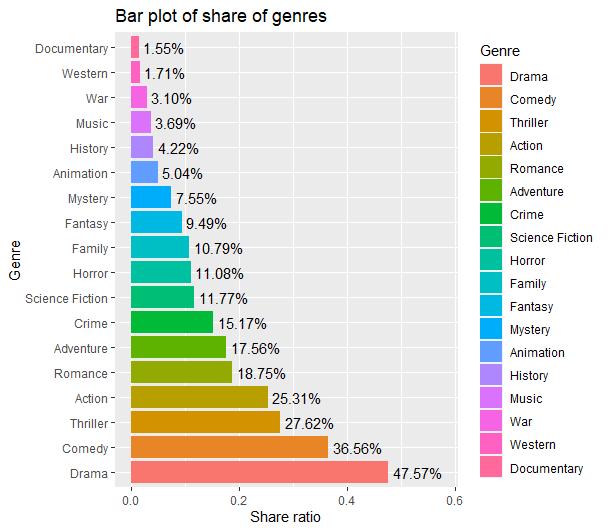
\includegraphics[scale=0.5]{share_genres.png}

Note that genres aren't mutually exclusive, that is, two different genres can correspond to a single movie. 
So the sum of percentages in the above graph will exceed 100.

From the bar graph, we can make the following conclusions:

\begin{itemize}
    \item `Drama' is the most common genre. Followed by `Comedy' and `Thriller'.
    This is not surprising, as these movies are all over.
    \item The least common genres are `Documentary', `Western', `War', `Music', and `History'; each have a share of less than 5\%.
    \item A (relatively new) genre that is becoming popular nowadays is missing from the dataset, `Slice of Life'. 
    This is because few websites categorize movies under this genre and TMDb apparently doesn't.
\end{itemize}

Let us now look at the relationship between different genres.
First, the share of movies having `Animation' as a genre.

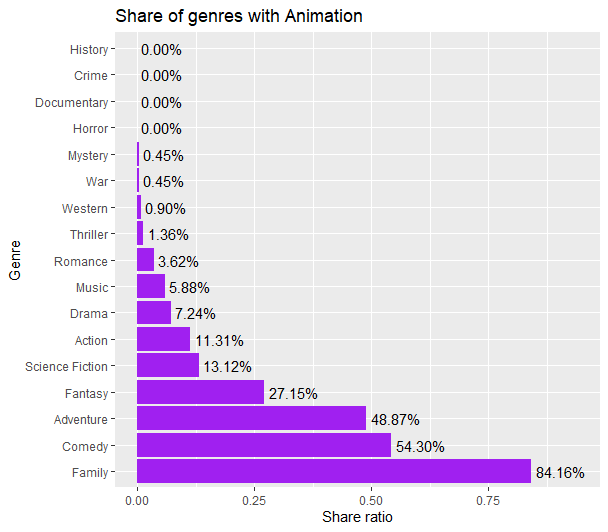
\includegraphics[scale = 0.5]{share_genres_animation.png}
\begin{itemize}
    \item From this, it is clear that most of the movies under \emph{Animation} also fall under \emph{Family}. This makes sense, 
    as (sadly) most of the animated movies are aimed towards kids. 
    \item Also, note that the sum of shares of `Family' and `Comedy' is greater than 1. 
    So we can conclude, 
    that there are animated movies that fall under both `Family' \emph{and} `Comedy'.
    \item We also see that there are no `Animated' movies that are also `Horror' or `Crime'.
\end{itemize}

For one more example, we look at the bar graph for `Romance'.

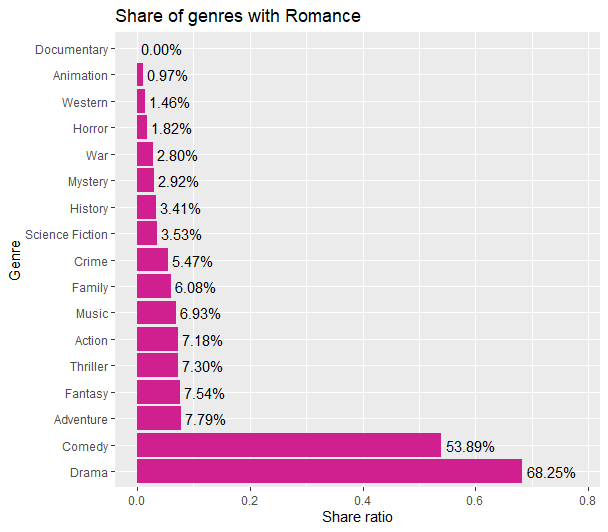
\includegraphics[scale=0.5]{share_genres_romance.png}

\begin{itemize}
    \item The relationship of `Romance' with `Drama' and `Comedy' is very prominent. 
    This may be attributed to the immence popularity of \emph{Rom-Coms}.
    \item There are no documentaries with genre `Romance' -- makes sense.
    \item Also, see that `Animation' is more common among various genres than 
    `Romance' -- which is only common with `Comedy' and `Drama', and not much with other genres.
    This makes sense, as unlike `Romance', `Animation' is not a hardcoded genre 
    and some (including yours truly) would argue that animation is more of a medium than a genre. 
\end{itemize}

Similarly, we can plot bar graphs for any genre to see its relationship with other genres.

\subsection{Genre vs Rating}

We first plot the boxplot of average rating by different genres. 

Before we proceed, note that for this section we will not use one hot encoding of genres, instead, we create multiple copy of rows for different genres, as this would enable us to easily plot boxplot and density plot.

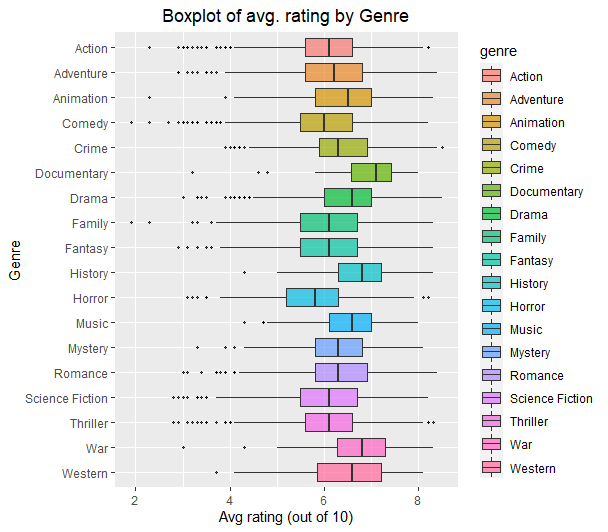
\includegraphics[scale=0.5]{boxplot_rating_genre.png}

\begin{itemize}
    \item Horror movies are generally rated lower, as compared to other genres.
    \item In contrast, documentaries are generally rated higher.
    \item `Drama' movies are generally rated higher than `Action' ones.
\end{itemize}

Let us now look at the probability density plot for each genre separately.

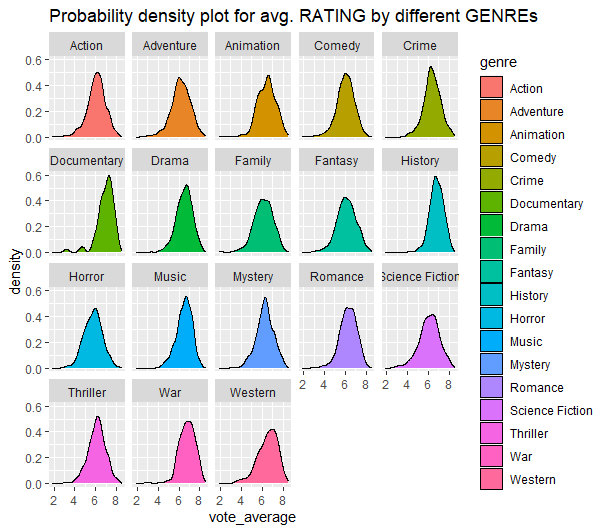
\includegraphics[scale=0.5]{density_rating_genres.png}

We are seeing Central Limit theorem in action. 

\subsection{Genre vs Budget}

There are a lot of movies with \texttt{budget} entry 0, or a small positive integer. 
We will remove them. In fact, for this, we only consider movies with a budget more than 100,000 USD. 
There are still more than 3600 unique movies in the filtered dataset; this is enough for us.

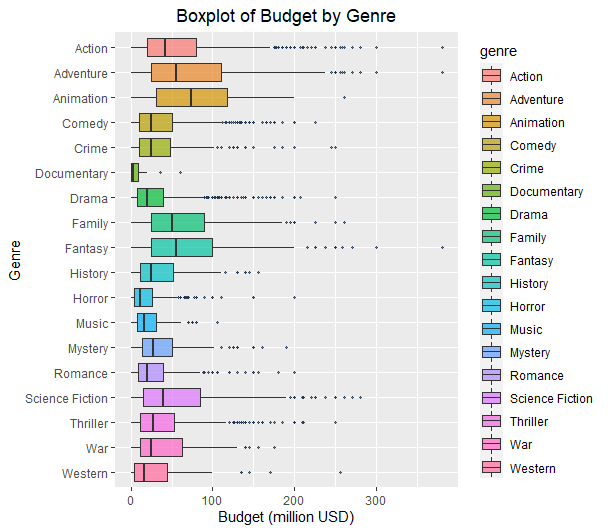
\includegraphics[scale=0.5]{boxplot_budget_genre.png}

\begin{itemize}
    \item Documentaries and horror movies tend to be cheaper than other genres.
    \item Drama movies are generally cheaper than Action movies but there are some high-budget drama movies as well.
    \item Most of the mega-budget movies fall under Action or Adventure. (Notice the outliers.)
\end{itemize}

\subsection{Rating vs Budget}

As in the previous section, we only consider movies with budget $\ge$ 100,000 USD.

We plot the graph of rating vs budget. 

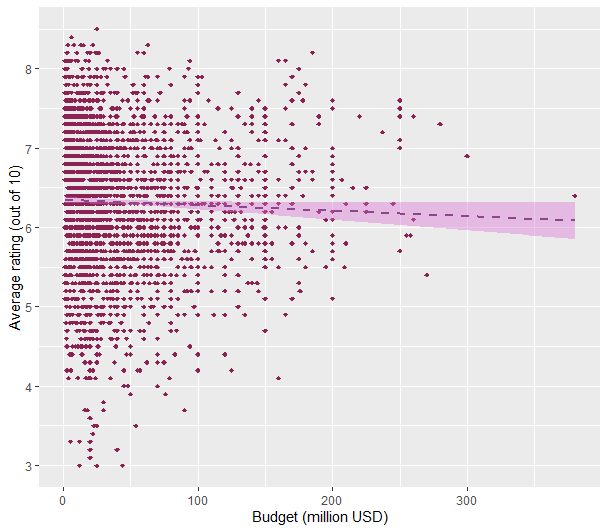
\includegraphics[scale=0.5]{rating_vs_budget.png}

\begin{itemize}
    \item Most of the movies have a budget of less than \$100 million.
    \item There seems to be no apparent relationship between budget and rating.
    \item All the movies with a rating of less than 4 don't have budget greater than 
    \$100 million. A very high budget somewhat ensures that the quality is not garbage.
\end{itemize}

\subsection{Rating vs Runtime}

We plot the graph of rating vs runtime.

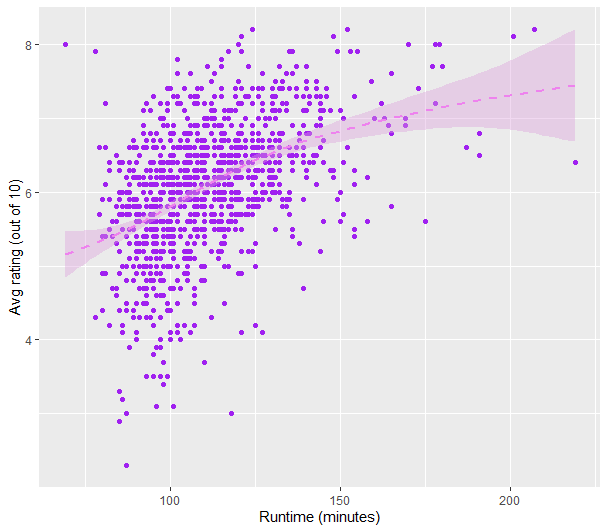
\includegraphics[scale=0.5]{rating_vs_runtime.png}

\begin{itemize}
    \item Most of the movies have a runtime $<$ 150 mins (2h30m).
    \item Longer movies tend to be rated higher.
\end{itemize}

\section{Summary}

From the entire visualisation process, the most important findings are noted below.

\begin{itemize}
\item It can be seen clearly that some of the genres are heavily interdependent.
\item For all the genres, ratings of movies tend to follow normal distribution. 
\item Documentaries and horror movies are generally cheaper than other genres.
\item There doesn't seem to be a relationship between ratings and budget. 
This is not surprising, as documentaries are generally rated higer, and horror movies lower, as compared to all other genres, even though both of them usually have a lower budget.
\item However, a very high budget somewhat ensures that quality is not subpar, as all the movies with budget $>$ \$100 million are all rated above 4.
\item Longer movies tend to be rated higher.
\end{itemize}

Some additional comments about the data:
\begin{itemize}
    \item More than 90\% of the movies in the dataset are English movies, however there are lots of great non-English movies out there. 
    In particular there are many French, Korean, any Japanese movies that are world famous. 
    \item The dataset also has a \texttt{release\_date} column. However, I didn't do any analysis using it as most of the movies in the dataset were released after 2000, and there are many famous movies from 20th century that weren't in the dataset.
    \item In conclusion, the dataset needs to be more diverse. 
\end{itemize}

\end{multicols}

\end{document}
